%%%% SEITENRAENDER, SCHRIFTGROESSE UND ZEILENABSTAND NICHT ABAENDERN => SONST GIBT ES PUNKTEABZUG
\documentclass[a4paper,11pt,singlespacing]{article}
% \usepackage[left=2.5cm,right=2.5cm,top=2.5cm]{geometry}
\usepackage{setspace}
\usepackage[utf8]{inputenc}
\usepackage[T1]{fontenc}
\usepackage{graphicx}
\usepackage[ngerman]{babel}
\usepackage{color}
\usepackage{wrapfig}
\usepackage{titleref}
\usepackage{hyperref}
\usepackage[rightcaption]{sidecap}
\usepackage{listings,xcolor}
\usepackage[numbers,round]{natbib}
\usepackage{textcomp}
\usepackage{float} % For image floating ([H] -> "here")

% Configuration
\sloppy
\graphicspath{ {images/} }

% Cover setup
\title{Systemadministration - Mailserver Honeypot zum analysieren von Spam}
\author{Manuel Adams 27470, Michael Ruf 27428, Mario Waizenegger 29608}

\begin{document}
\setlength{\parindent}{0ex} % Absatzeinrückung verhindern
\pagenumbering{roman}

\maketitle

\begin{abstract}
Heutzutage wird viel \nameref{itm:Spam} verschickt. Einiges davon wird erkannt und gefiltert.
Um die Analyse von Spam-Nachrichten und deren Versender zu ermöglichen, wird ein Mailserver \nameref{itm:Honeypot} aufgesetzt.
Dieser soll \nameref{itm:Spam}-Nachrichten erhalten können, sowie als offener Verteiler für Spammer verfügbar sein.
\end{abstract}

\newpage

% Table of contents
\tableofcontents

\newpage
\pagenumbering{arabic}

% Content
\section{Einleitung}\label{sec:Einleitung}
	% NOTE "Wir" erlaubt
	Warum \nameref{itm:Spam} versandt wird ist vielen Menschen ein Rätsel.
	Das wirft die Fragen auf, wer Spam versendet und was die Beweggründe von Spammern sind.
	Wie geht man mit Spam um und was passiert wenn man auf \nameref{itm:Spam} reagiert?
	Ein \nameref{itm:Spam} \nameref{itm:Honeypot} bietet die Möglichkeit diese Fragen zu analysieren und die nötigen Daten zu erheben.
	% NOTE Warum lohnt sich das?
	\\
	Da die Methoden von erfolgreichen Spammern nicht dokumentiert sind, ist das Bekanntmachen des "`\nameref{itm:OpenRelay}"'"~Servers schwierig.
	Zudem ist es zeitaufwendig die eigenen Mail-Adressen unter Spammern bekannt zu machen und viele authentische Spam-Mails in kurzer Zeit zu erhalten eine Herausforderung.
	% NOTE Man kann man beim Ergebnis nochmal Stellungnahme hierzu nehmen oder den Text hier ergänzen
	% -----
	% - Wirtschaftlichkeit
	% - Andere Beweggründe
	% - Findet man Informationen über Systeme, von denen Spam verschickt wird?
	% - Werden die Nachrichten generiert? (Bots)

	\subsection{Ziel der Arbeit}\label{sec:EinleitungZiel}
		Es soll durch einen Mailserver Honeypot Erkenntnisse über Herkunft, Zweck und Zielgruppe von \nameref{itm:Spam} Nachrichten erhalten werden.
		Zusätzlich soll erarbeitet werden welche weiteren nützlichen Informationen man den Mails entnehmen kann.
		Durch diese Informationen soll die Motivation von Spammern besser verstanden und entsprechende Vorkehrungen zum Schutz ermöglicht werden.
		% NOTE Was wird genau analysiert
	
	\subsection{Vorgehensweise}\label{sec:EinleitungVorgehensweise}
		Um den Honeypot zu realisieren muss der Mail-Dienst aus dem Internet zugänglich sein.
		Dieser besteht hierbei aus Ausgangsserver und Eingangsserver.
		Hierzu werden auf einer \nameref{itm:VirtuelleMaschine} die Dienste in \nameref{itm:Container}n aufgesetzt.
		Aus Sicherheitsgründen muss die \nameref{itm:VirtuelleMaschine} ins interne Netz abgeschottet sein.
		Der Aufbau ist in \autoref{fig:Hierarchy} visualisiert.

		\begin{figure}[H]
			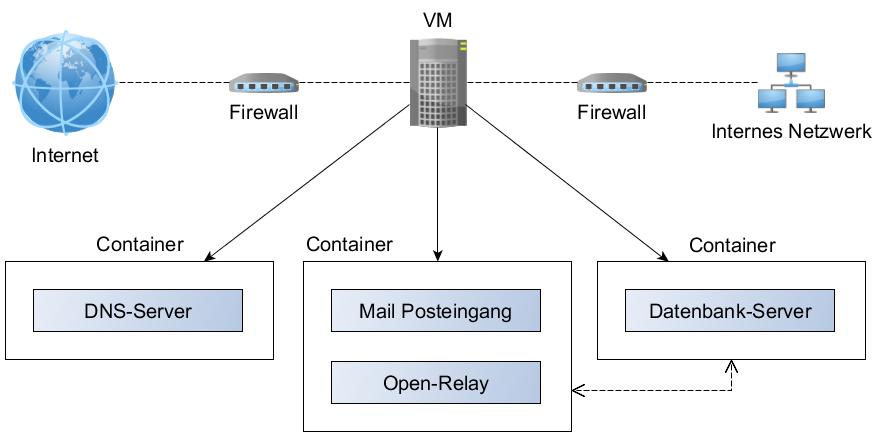
\includegraphics[width=\linewidth]{2-Hierarchy.png}
			\caption{Netzwerkstruktur}
			\label{fig:Hierarchy}
		\end{figure}

		Um den Eingangsserver zu realisieren sind folgende Aufgaben erforderlich:
		\begin{enumerate}
			\item Mail Eingangsserver bereitstellen und konfigurieren
			\item \nameref{itm:DNS} Server einrichten um realistische E-Mail-Adressen bereitzustellen
			\item Bei möglichst vielen Diensten mit unterschiedlichen Mailadressen registrieren
			\item Mails analysieren indem per Script geprüft wird, ob sich Informationen  über den Versender ermitteln lassen.
		\end{enumerate}

		Den Ausgangsserver betreffend sind folgende Aufgaben erforderlich:
		\begin{enumerate}
			\item Mail Ausgangsserver bereitstellen und konfigurieren
			\item Als "`\nameref{itm:OpenRelay}"' im Internet durchsickern lassen
			\item Eingehende Mails tatsächlich weiterleiten
			\item Mails analysieren
		\end{enumerate}

	\subsection{Aufbau der Arbeit}\label{sec:EinleitungAufbau}
		\begin{itemize}
			\item In Abschnitt 1 werden die nötigen Grundbegriffe zum Verständnis abgesteckt.
			\item In Abschnitt 2 wird das Projekt und die Zielsetzung zusammengefasst.
			\item In Abschnitt 3 geht es die Problemstellung des Projekts.
			\item In Abschnitt 4 werden die zu erarbeitenden Ziele genannt.
			\item In Abschnitt 5 werden mögliche technische Lösungen zur Problemstellung benannt und bewertet.
			\item In Abschnitt 6 werden die am besten passenden Lösungen aus Abschnitt 5 genannt.
			\item In Abschnitt 7 wird beschrieben wie die tatsächliche Umsetzung anhand der technischen Lösungen aus Abschnitt 6 aussieht.
			\item In Abschnitt 8 wird das Projekt nochmals zusammengefasst und ein Fazit gezogen.
		\end{itemize}

\newpage

\section{Grundbegriffe}\label{sec:Grundbegriffe}
	Die folgenden Begriffsdefinitionen und Unterscheidungen sind zum einen zur Verdeutlichung, wie Begriffe in dieser Arbeit verstanden werden und um Fachbegriffe zu erklären.

	\begin{description}
	\item[Spam\label{itm:Spam}]\hfill \\
		Als Spam oder Junk werden unerwünschte, in der Regel auf elektronischem Weg übertragene Nachrichten[...] bezeichnet, die dem Empfänger unverlangt zugestellt werden und häufig werbenden Inhalt enthalten. Dieser Vorgang wird Spamming oder Spammen genannt, der Verursacher Spammer.\cite{Spam}
	\item[Honeypot\label{itm:Honeypot}]\hfill \\
		Sicherheitstechnisch scheinbar verwundbares Computerprogramm, das Computerviren, -würmer und Trojaner anlockt, um sie zu registrieren und unschädlich zu machen.\cite{Honeypot}
	\item[Open-Relay\label{itm:OpenRelay}]\hfill \\
		Ein \nameref{itm:SMTP}-Relay-Server der durch unzureichende Sicherheitskonfiguration auch Mails weiterleitet bei denen er weder für die Absender- noch für die Zieladresse zuständig ist, wird als "`Open relay"' bezeichnet.\cite{SMTP-Relay-Server}
	\item[Virtuelle Maschine (VM)\label{itm:VirtuelleMaschine}]\hfill \\
		Eine VM ist eine Kapselung eines Rechnersystems auf Softwareebene. Dadurch lässt sich eine Rechnerarchitektur in einem Container simulieren. \cite{VM}
	\item[Blacklist \label{itm:Blacklist}]\hfill \\
		Eine Blacklist oder "`schwarze Liste"' enthält eine Auflistung von Daten, die von einem Prozess ausgeschlossen werden solle. Das Gegenteil dazu ist eine Whitelist. \cite{Blacklist}
	\item[Container\label{itm:Container}]\hfill \\
		Containervirtualisierung ist eine Methode, um mehrere Instanzen eines Betriebssystems isoliert voneinander auf einem Hostsystem zu betreiben.\cite{Container}
	\item[DNS\label{itm:DNS}]\hfill \\
		Das Domain Name System (DNS) ist einer der wichtigsten Dienste in vielen IP-basierten Netzwerken. Seine Hauptaufgabe ist die Beantwortung von Anfragen zur Namensauflösung.\cite{DNS}
	\item[DKIM\label{itm:DKIM}]\hfill \\
		DKIM (DomainKeys Identified Mail) ist eine Methode der E-Mail-Authentifizierung. DKIM fügt Ihren Mails eine Signatur hinzu, die Ihrer Domain zugeordnet ist und bei allen ausgehenden E-Mails genutzt wird. Das Verwenden eines DomainKey ist eine Technik[...], die das Fälschen des Absenders einer E-Mail erschweren soll.\cite{DKIM}
	\item[Hook\label{itm:Hook}]\hfill \\
		Hook (englisch für Haken, auch Einschubmethode genannt) bezeichnet in der Programmierung eine Schnittstelle, mit der fremder Programmcode in eine bestehende Anwendung integriert werden kann, um diese zu erweitern, deren Ablauf zu verändern oder um bestimmte Ereignisse abzufangen.\cite{Hook}
	\item[Catch-All-Mail-Adressen\label{itm:Catch-All-Mail}]\hfill \\
		Die Catch-All-Weiterleitung bewirkt, dass alle E-Mails an Zieladressen der Form <beliebige gültige Zeichenfolge>@Domain in der gleichen Mailbox zusammenlaufen.\cite{Catch-All-Mail}
	\item[Crawler\label{itm:crawler}]\hfill \\
		A Web crawler, sometimes called a spider or spiderbot and often shortened to crawler, is an Internet bot that systematically browses the World Wide Web \cite{crawler}
	\item[HTML\label{itm:HTML}]\hfill \\
		Hypertext Markup Language (HTML) is the standard markup language for documents designed to be displayed in a web browser.\cite{HTML}
	\item[Virtueller privater Server (VPS)\label{itm:VPS}]\hfill \\
        	Definiert ist der Virtual Private Server als ein virtueller Webserver auf der Basis eines physikalischen Servers.
		Der leistungsstarke physikalische Server wird unterteilt in mehrere Virtual Private Server.\cite{VPS}
	\item[Provider\label{itm:Provider}]\hfill \\
		Ist ein Unternehmen, das Dienstleistungen im Bereich EDV und Internet anbietet. \cite{provider}
	\item[IMAP\label{itm:IMAP}]\hfill \\
		Das Internet Message Access Protocol (IMAP) ist ein Client-Server Protokoll, dass das Empfangen und Versenden von E-Mails über einen Mail-Server ermöglicht. Es synchronisiert alle Änderungen zurück auf den Server, sodass auf allen Endgeräten die gleichen Daten zugreifbar sind. \cite{imap}
	\item[POP3\label{itm:POP3}]\hfill \\
		Das Post Office Protocol 3 (POP3) ist wie \nameref{itm:IMAP} zum  Empfangen und Versenden von E-Mails. Allerdings löscht dieses Protokoll die MAils auf dem Server nachdem diese vom Server auf den Client heruntergeladen wurden. Somit ist keine Synchronisierung zwischen verschiedenen Endgeräten möglich.\cite{pop3}
	\item[SMTP\label{itm:SMTP}]\hfill \\
		Das Simple Mail Transfer Protocol (SMTP) dient in IP-Netzen zum weiterleiten von E-Mails zwischen den einzelnen Servern. \cite{smtp}
	\item[SSL\label{itm:SSL}]\hfill \\
		Secure Socets Layer soll die Internetverbindung absichern und sensible Daten, die zwischen zwei Systemen übertragen werden, schützen. Dabei sorgen Verschlüsselungsalgorithmen bei der Datenübertragung dafür diese zu kodieren, um das Mitlesen zu verhindern. \cite{ssl}
	\item[Traffic\label{itm:Traffic}]\hfill \\
		Unter Traffic oder auch Datenverkehr wird der Datenfluss in Netzwerken verstanden. \cite{traffic}
	\item[MX-Rekord\label{itm:MX-Rekord}]\hfill \\
		Ein MX-Rekord definiert unter welchem Domain Name ein Mail-Server einer Domain erreicht werden kann. \cite{mxRekord}
	\item[SQL\label{itm:SQL}]\hfill \\
		SQL ist eine Datenbanksprache die es ermöglicht in relationalen Datenbanken Datenstrukturen zu verwalten. \cite{sql}
	\item[Tracking\label{itm:Tracking}]\hfill \\
		Eine Tracking URL beinhaltet bestimmte ID´s oder Parameter, über die der Weg des Nutzers dieses Links beim Aufruf verfolgt werden kann. \cite{tracking}
	\end{description}

\newpage


\section{Problemstellung}\label{sec:Problemstellung}
	Spammer dokumentieren ihre Arbeit eher nicht.
	Daher sind deren Vorgehensweisen unklar.
	Um einen Einblick zu erhalten sind nachfolgende Probleme zu lösen.
	% Unterpunkte:
	% - Sehr konkret
	% - Forschungsfrage festnageln

	\subsection{Konfiguration}\label{sec:ProblemstellungKonfiguration}
		Um einen reibungslosen Ablauf zu gewährleisten muss der Mailserver in der Lage sein Mails zu empfangen.
		Empfangene Mails sollen persistiert werden.
		Eine hohe Verfügbarkeit ist hier von Vorteil.
		\\
		Der Server soll zudem als \nameref{itm:OpenRelay} dienen.
		Hierfür muss dieser so konfiguriert werden, dass eingehende externe Mails nicht abgewiesen werden.
		\\
		Um die Mails abzulegen bietet sich ein Datenbank Server an.
		Die Daten auf dem Mail-Server dürfen dadurch jederzeit verworfen werden und Änderungen am Mailserver können ohne Auswirkung auf vorhandene Daten umgesetzt werden.

	\subsection{Mail-Adressen verteilen}\label{sec:ProblemstellungMailsVerteilen}
		Damit authentische Spam Mails erhalten werden, müssen die E-Mail-Adressen echt wirken.
		Um das zu erreichen müssen die Adressen
		\begin{itemize}
		\item möglichst lange, also möglichst früh in Verwendung sein,
		\item aktiv benutzt werden
		\item und bei möglichst vielen Diensten benutzt werden.
		\end{itemize}
		Es soll identifiziert werden können von welchem Dienst eine Mail eingeht.
		Zudem bietet es sich an auf eingehende Spam-Mails zu reagieren indem man bspw. auf vorhandene Links klickt, da \nameref{itm:Tracking}-Links enthalten sein können oder auf die Mail antwortet.

	\subsection{Open-Relay Publizieren}\label{sec:ProblemstellungPublizieren}
		Der \nameref{itm:Honeypot} muss bei Spammern als unsicher wirkender \nameref{itm:OpenRelay} und guter Spamverteiler bekannt werden.
		Im Internet muss die Adresse des Servers hierzu so verteilt werden, dass Spammer darauf aufmerksam werden.
		Nach Möglichkeit sollte der Server nicht in einer \nameref{itm:OpenRelay} \nameref{itm:Blacklist} auftauchen, da er ansonsten nicht mehr nützlich für Spammer ist.

	\subsection{Analysieren}\label{sec:ProblemstellungAnalysieren}
		Es soll erarbeitet werden, welche Aspekte von Spam analysiert werden können:
		\begin{itemize}
		\item Kann man Informationen über das System von dem gesendet wurde erhalten?
		\item Könnte man den Weg den die \nameref{itm:Spam}"~Mails vom Versender bis zum Empfänger genommen haben zurückverfolgen?
		\item Inwiefern lässt sich der Inhalt der Mail auf Schreibweise, Textinhalt oder auch Anhänge analysieren?
		\end{itemize}

\newpage


\section{Anforderungsanalyse}\label{sec:Anforderungsanalyse}
	Folgende Anforderungen \textbf{MÜSSEN}/\textbf{SOLLEN}/\textbf{KÖNNEN} erarbeitet werden, damit die \nameref{sec:Problemstellung} gelöst werden kann:

	\begin{enumerate}
	\item
		Der Mail"~Server \textbf{MUSS} die Mails empfangen können.
		(\ref{sec:ProblemstellungKonfiguration})
	\item
		Es \textbf{MUSS} auf eingehende Spam"~Mails reagiert werden.
		(\ref{sec:ProblemstellungMailsVerteilen})
	\item
		Es \textbf{MUSS} erarbeitet werden, welche Aspekte von Spam analysiert werden können.
		(\ref{sec:ProblemstellungAnalysieren})
	\item
		Der Mail"~Server \textbf{SOLL} als \nameref{itm:OpenRelay} dienen.
		Diese Mails sollen nicht versendet, sondern lediglich persistiert werden.
		(\ref{sec:ProblemstellungKonfiguration})
	\item
		Die Mail"~Adressen \textbf{SOLLEN} echt wirken.
		(\ref{sec:ProblemstellungMailsVerteilen})
	\item
		Die Adresse des \nameref{itm:OpenRelay} Servers \textbf{SOLL} bei Spammern bekannt werden.
		(\ref{sec:ProblemstellungPublizieren})
	\item
		Die Daten \textbf{KÖNNEN} auf einem Datenbankserver abgelegt werden, welcher über Mail"~"`\nameref{itm:Hook}s"' die Daten bekommt.
		(\ref{sec:ProblemstellungKonfiguration})
	\item
		Zur Identifizierung \textbf{KANN} sich bei den Diensten mit einer "`\nameref{itm:Catch-All-Mail}"' mit einem Präfix für den jeweiligen Dienst registriert werden.
		(\ref{sec:ProblemstellungMailsVerteilen})
	\item
		Der Server \textbf{KÖNNTE} nicht in einer \nameref{itm:OpenRelay} \nameref{itm:Blacklist} auftauchen.
		(\ref{sec:ProblemstellungPublizieren})
	\end{enumerate}

\newpage


\section{Lösungsvorschläge}\label{sec:Lösungsvorschläge}
	Nachfolgende Lösungsvorschläge werden recherchiert und auf ihre Eignung für die Arbeit überprüft.

	\subsection{Provider}\label{sec:Provider}
		Für das Hosting des Mailserver-\nameref{itm:Honeypot}s muss ein geeigneter \nameref{itm:Provider} für einen \nameref{itm:VPS} gefunden werden, welcher die Anforderungen
		\begin{itemize}
			\item anonymes Hosting, also kein Bezug zu Personen inklusive Domain mit Whois-Schutz,
			\item ausreichend Speicher für mehrere Docker-Instanzen sowie den empfangenen Spam-Mails,
			\item ein Domain sowie die Möglichkeit zur DNS Administration und
		\end{itemize}
		erfüllt.\\
		Hierfür kann eine \nameref{itm:VirtuelleMaschine} im Rechenzentrum der Hochschule Ravensburg-Weingarten oder ein externer \nameref{itm:Provider} angemietet werden.

	\subsection{Host-OS}\label{sec:Host-Maschine}
		Das Betriebssystem des \nameref{itm:VPS} hat die Anforderung mit möglichst wenig Hardware-Ressourcen sowie ohne GUI lauffähig zu sein.
		Nachfolgende Systeme werden betrachtet und evaluiert.

		\subsubsection{OpenBSD}\label{sec:OpenBSD}
			OpenBSD ist kompakt und übersichtlich.
			Da das System eine auf Sicherheit ausgelegte UNIX-Distribution ist, könnten Spammer möglicherweise abgeschreckt werden den Mail-Relay-Server zu verwenden. \cite{openBSD}

		\subsubsection{Debian}\label{sec:Debian}
			Debian ist weit verbreitet, einfach zu konfigurieren und freies Betriebssystem.
			Da Debian wenig Hardware Ressourcen braucht und Distributionen ohne GUI existieren, eignet es sich als Server-Betriebssystem. \cite{debianVerbreitet} \cite{debian}

	\subsection{Virtualisierung}\label{sec:Virtualisierung}
		Um die einzelnen Dienste von einander zu trennen soll eine Virtualisierung stattfinden.
		Nachfolgend werden Varianten dazu überprüft.

		\subsubsection{Verwendung der Host-Maschine}\label{Verwendung der Host-Maschine}
			Die direkte Verwendung der Host-Maschine spart den Aufwand der Virtualisierungsumsetzung.
			Sollte jedoch Schadsoftware auf die Host-Maschine gelangen können gro{\ss}e Schäden entstehen.
			Wenn ein Dienst konfiguriert oder angepasst wird ist der Dienst während dieser Zeit nicht erreichbar.

		\subsubsection{Virtuelle-Maschine}\label{Virtual-Maschine}
			Durch den Einsatz Virtueller-Maschinen für die Mailserver ist die Host-Maschine vor Schadsoftware geschützt.
			Backups der kompletten virtuellen Maschine können sehr groß sein und es dauert unter Umständen lange diese im Fehlerfall wieder einzuspielen.

		\subsubsection{Docker}\label{Docker}
			Docker-\nameref{itm:Container} sind gegen das Host-System abgeschottet. Falls Schadsoftware in den Container gelangt, kann diese auf dem Host-System keinen Schaden verursachen.
			Docker-\nameref{itm:Container} sind mit wenig Aufwand reproduzierbar und austauschbar. Au{\ss}erdem können diese leicht auf andere Host-System portiert werden.
			Es ist mit Docker möglich Ports an die einzelnen Container weiter zu leiten. Dadurch können Dienste mehrfach ausgeführt werden.
			Mit der Konfiguration eines Docker-\nameref{itm:Container}s in einer externen Konfigurationsdatei (z.B. in der docker-compose.yml), ist diese automatisch dokumentiert, kann versioniert werden und ist folglich für Gruppenprojekte geeignet. (siehe z.B. in \autoref{lst:Maileingangsserver})
			\nameref{itm:Container} können schnell herunter und wieder hochgefahren werden, wodurch das Testen von neuen Konfigurationen sehr effizient wird.

	\subsection{Maildienste}\label{sec:Mailserver}
		Um Spam-Mails zu empfangen sowie einen \nameref{itm:OpenRelay} anbieten zu können, soll ein einfach zu konfigurierender Mailserver gefunden werden.
		Als Eingangsserver und als Ausgangsserver für den \nameref{itm:OpenRelay} kommen verschiedene Mailserver in Frage von denen nachfolgend eine Auswahl geprüft wird.

		\subsubsection{Postfix}\label{sec:Postfix}
			Postfix ist ein Mailserver für UNIX der mit Fokus auf Sicherheitsaspekte entwickelt wurde.
			Das Tool ist als Open-Source Projekt frei verfügbar und soll eine Alternative zu Sendmail bieten.
			\cite{postfix}

		\subsubsection{Docker Mailserver}\label{sec:FullstackDockerMailserver}
			Es gibt Docker-Images, welche komplette Mailserver mit ihrer Konfiguration bereitstellen.
			Nachfolgend wird eines dieser von \href{https://github.com/tomav/docker-mailserver}{GitHub} betrachtet.
			Funktionen wie \nameref{itm:SMTP}, \nameref{itm:IMAP}, Antispam, Antivirus und viele weitere sind in diesem Image enthalten.
			Intern verwendet der Container ebenso \nameref{sec:Postfix} und \nameref{sec:Dovecot} sowie LDAP Authentifizierung.
			Bei der Verwendung dieses Mailservers zum Spam-Empfang müssen die Anti-Spam-Funktionen deaktiviert bzw. so konfiguriert werden um Spam zu erhalten.

		\subsubsection{OpenSMTPD}\label{sec:OpenSMTPD}
			Ist ein frei verfügbarer Unix basierter Mailserver von \nameref{sec:OpenBSD}, der durch seine einfach gehaltene Konfiguration überzeugt.
			Es werden nur wenige Files benötigt um einen Mailserver aufzusetzen.
			\cite{openSMTPD}

		\subsubsection{Dovecot}\label{sec:Dovecot}
			Dovecot ist ein sicherer Open-Source Dienst mit Unterstützung von \nameref{itm:IMAP} und \nameref{itm:POP3} für UNIX Distributionen.
			Das Tool eignet sich sowohl für einfach gehaltene, aber auch für grö{\ss}ere komplexere Konfigurationen.
			Es ist einfach aufzusetzen und erfordert dabei keine besondere Administration.
			Dovecot ist schnell und benötigt nur wenig Arbeitsspeicher. \cite{dovecot}

\newpage


\section{Auswahl Lösung anhand Anforderungen}\label{sec:AuswahlLösungAnhandAnforderungen}
	Nachfolgend werden die Lösungsvorschläge bewertet und die zu verwendeten Techniken werden aufgrund ihrer Eignung benannt.

	\subsection{Provider}\label{sec:AuswahlLösungProvider}
		Bei der \nameref{itm:Provider} Auswahl wurde eine \nameref{itm:VirtuelleMaschine} beim Hochschulrechenzentrum beantragt, da sich dies bei einer Arbeit im Rahmen des Studiums anbietet.
		Nachfolgend wird eine \nameref{itm:VirtuelleMaschine} im \href{https://www.hs-weingarten.de/web/rechenzentrum}{Rechenzentrum} der Hochschule und externe \nameref{itm:Provider} verglichen und bewertet.
		
		\subsubsection{Hochschulrechenzentrum}\label{sec:AuswahlLösungDMZHochschulrechenzentrum}
			Die Tatsache, dass keinerlei Rückschlüsse auf die Hochschule gezogen werden dürfen, erschwert den Antrag auf eine \nameref{itm:VirtuelleMaschine} im Hochschulrechenzentrum.
			Eine Verbindung zur Hochschule könnte die Glaubwürdigkeit des \nameref{itm:OpenRelay} einschränken.
			Zudem befürchtet die Hochschule einen Eintrag der IP-Adressen in Spam-Blacklists.

			Folglich wurde der Antrag über eine \nameref{itm:VirtuelleMaschine} im Rechenzentrum der Hochschule abgelehnt.
			Das Rechenzentrum ist der Meinung, dass es aus sicherheitsrelevanten Gründen für dieses Projekt keine \nameref{itm:VirtuelleMaschine} zur Verfügung stellen kann.
			Aus diesem Grund kann für die Umsetzung nur ein externer \nameref{itm:Provider} in Betracht gezogen werden.

		\subsubsection{Externer Provider}\label{sec:AuswahlLösungExterneProvider}
			Anhand der Kriterien wie in \autoref{sec:Provider} beschrieben wurde ein Hosting-\nameref{itm:Provider} für den \nameref{itm:VPS} ausgewählt.
			Weitere berücksichtige Merkmal waren
			\begin{itemize}
				\item ein akzeptables Preisleistungsangebot,
				\item eine simple Konfigurationsoberfläche für den DNS, sowie
				\item die Verfügbarkeit von Debian als Betriebssystem (siehe \autoref{sec:AuswahlLösungDMZHochschulrechenzentrum}).
			\end{itemize}		

	\subsection{Host-OS}\label{sec:AuswahlLösungHost-Maschine}
		Windows und OpenBSD als Betriebssystem entfallen aus den in \autoref{sec:Host-Maschine} erwähnten Gründen.
		Auf dem \nameref{itm:VPS} soll folglich Debian als Betriebssystem laufen.
		Der Server wird von einem externen \nameref{itm:Provider} vorkonfiguriert bereitgestellt.
		Im Projektverlauf müssen nur noch Änderungen der bestehenden Konfiguration vorgenommen werden.

	\subsection{Virtualisierung}\label{sec:AuswahlLösungVirtualisierung}
		Aufgrund der guten Wartbarkeit und Änderbarkeit wird im Projekt zur Virtualisierung Docker verwendet.
		Jeder Dienst soll hierfür in einem eigenen Container realisiert werden, sodass diese einfach ausgetauscht werden können.

	\subsection{Maildienste}\label{sec:AuswahlLösungMailserver}
		Aus zeitlichen Gründen für die Umsetzung des Projekts, soll sowohl für den Eingangs-Mailserver als auch für das \nameref{itm:OpenRelay} ein Tool gewählt werden, das eine kompakte Einrichtung in einem Docker-\nameref{itm:Container} bietet.
		Aus diesem Grund bietet es sich an für die beiden Anwendungsfälle unterschiedliche Mailserver aufzusetzen.

		\subsubsection{Postfix}\label{sec:AuswahlLösungPostfix}	
			Da Postfix im \nameref{sec:FullstackDockerMailserver} enthalten ist bietet dieser eigenständig weniger Features.
			Um die gleichen Vorteile und eine sichere Authentifizierung einzurichten ist damit zusätzlicher Konfigurationsaufwand erforderlich.
			Daher wird auf eine Konfiguration für Postfix alleinstehend verzichtet.

		\subsubsection{Docker Mailserver-Image}\label{sec:AuswahlLösungVorkonfigurierterDockerMailserver}
			Das Docker-Image kann von \href{https://github.com/tomav/docker-mailserver}{GitHub} heruntergeladen werden.
			Der Container muss dann nur noch konfiguriert werden und beinhaltet alle nötigen Komponenten um Mails empfangen und senden zu können. \cite{fullstackDockerMailserver}
			Auch das einrichten der \nameref{itm:Catch-All-Mail}-Adresse ist problemlos möglich.

			Da die Grundkonfiguration des Containers sinnvoll gewählt wurde sind nur wenige Schritte nötig um den Spam-Empfang zu ermöglichen.
			Aus diesem Grund bietet sich der \nameref{sec:FullstackDockerMailserver} an.

		\subsubsection{OpenSMTPD}\label{sec:AuswahlLösungOpenSMTPD}
			Da der \nameref{sec:OpenSMTPD} Mailserver eine kompakte und übersichtliche Konfiguration bietet, ist dieser für den \nameref{itm:OpenRelay} geeignet.
			In den Konfigurationsfiles kann sehr einfach angegeben werden, dass der Server Mails von allen Adressen an beliebige Zieladressen weiterleitet.
			Damit muss nur noch sicher gestellt werden, das diese Spam-Mails nicht wirklich nach au{\ss}en gelangen, sondern lediglich empfangen und gespeichert werden.

		\subsubsection{Dovecot}\label{sec:AuswahlLösungDovecot}
			Dovecot bietet eine Möglichkeit Mails über \nameref{itm:IMAP} oder \nameref{itm:POP3} abzuholen. \citep{dovecot}
			Dieser kann für den \nameref{itm:OpenRelay} eingesetzt werden, um die ausgehenden Mails vom Mailserver zu persistieren.
			Dadurch können die im Dovecot gespeicherten Mails via \nameref{itm:IMAP} oder \nameref{itm:POP3} bezogen und analysiert werden.

		\subsubsection{Mailserver Auswahl}\label{sec:MailserverAuswahl}	
			Für den Eingangsserver ist der \nameref{sec:FullstackDockerMailserver} die geeignete Methode um schnell das gewünschte Ergebnis zu erzielen.
			Damit kann innerhalb kurzer Zeit mit der Verbreitung der Adressen zum Spam-Empfang begonnen werden.

			Der \nameref{itm:OpenRelay} soll mit \nameref{sec:OpenSMTPD} umgesetzt werden.
			\nameref{sec:Dovecot} soll dabei als Dienst zum Abgreifen der Mails dienen, die über den \nameref{itm:OpenRelay} eingehen.

\newpage


\section{Umsetzung}\label{sec:Umsetzung}
	Anhand der im vorherigen Abschnitt benannten einzusetzenden Techniken wird im folgenden die praktische Umsetzung beschrieben.
	
	\subsection{Provider Registrierung}\label{sec:ProviderRegistrierung} 
		Wie bereits in \autoref{sec:AuswahlLösungProvider} erwähnt, wird die benötigte \nameref{itm:VirtuelleMaschine} für die Umsetzung des Projekts bei einem externen \nameref{itm:Provider} gehostet.
		Nach Absprache mit dem betreuenden Professor, wurde die Übernahme der Kosten für die Anmietung eines Virtuellen Servers inklusive einer Domain von der Hochschule bestätigt.

		Bei der Registrierung wurde der kleinste Virtuelle Server gewählt, der mit einer virtuellen CPU, 2GB Arbeitsreicher sowie 20GB SSD Festplatte für das geplante Projekt ausreichend ist.
		Weitere Features wie ungedrosselter \nameref{itm:Traffic} sind für den geplanten Spam-Empfang ebenfalls von Vorteil.
		
		Für die Domain haben wir uns für einen unauffälligen Namen entschieden, sodass Spammer keinen Verdacht schöpfen.
		Der Provider bietet einen Whois-Schutz, womit die Domain keinen Bezug zum Besitzer hat.
		
	\subsection{Host Einrichtung}\label{sec:UmsetzungHostEinrichtung}
		Nachfolgende Schritte wurden auf der angemieteten Maschine ausgeführt.
		
		\subsubsection{DNS Einträge}\label{sec:DNSEinträge}
			Im Control-Panel der Domain, wird für den Eingangsserver ein DNS-Eintrag für die \texttt{Mail} angelegt, dieser \nameref{itm:MX-Rekord} zeigt auf die IP-Adresse des Servers.
			Zusätzlich zu den DNS-Einträgen für die Mailserver wird noch ein Eintrag für die Website \href{https://babedibubip.de}{babedibubip.de} erstellt.

		\subsubsection{Docker}\label{sec:DockerAufsetzen}
			Bevor die verschiedenen \nameref{itm:Container} konfiguriert werden können, muss Docker installiert sein. Dies kann wie auf der  \href{https://docs.docker.com/install/linux/docker-ce/debian/}{Website} beschrieben, für  Debian nachgemacht werden.
			Danach können Docker-Images einfach bezogen und eingebunden werden.
			Die Weiterleitung der Anfragen an die unterschiedlichen Mailserver erfolgt anschlie{\ss}end bei den Konfigurationen in den Docker-\nameref{itm:Container}n.
	
	\subsection{Eingangsserver}\label{sec:UmsetzungEingangsserver}
		Der Mail-Eingangserver besteht aus den Komponenten Mailserver und dem Datenbank Script.
		Des weiteren wird noch ein \nameref{itm:SSL}-Zertifikat benötigt welches die Authentizität des Mailservers sicherstellt und eine \nameref{itm:SQL}-Datenbank um die Mails zu persistieren.
		Im folgenden Abschnitt wird die Konfiguration dieser Docker-\nameref{itm:Container} vorgenommen.

		\subsubsection{Mail-Container Konfiguration}\label{Mail-In-Container}
			Wie in \autoref{sec:AuswahlLösungVorkonfigurierterDockerMailserver} beschrieben wird das Image verwendet und wie in \autoref{lst:Maileingangsserver} konfiguriert.
			Um Mails zu Empfangen und per \nameref{itm:IMAP} über einen Mail-Client beziehen zu können werden die folgende Ports benötigt:
			\begin{itemize}
				\item 25 für TLS \nameref{itm:SMTP}
				\item 143 TLS \nameref{itm:IMAP}
				\item 587 TLS default mail submission port
				\item 993 SSL \nameref{itm:IMAP}
			\end{itemize}
			Da für den Erhalt von Spam dieser nicht gefiltert werden soll, werden die Module \textit{Spamassassin}, \textit{Clamav}, \textit{Fail2ban}, \textit{Postgrey} und \textit{Spoof-Protection} deaktiviert.
			
		\subsubsection{SSL Konfiguration}\label{SSL-Container}
			Die \nameref{itm:SSL}-Zertifikate werden über einen Container bezogen, dieser wurde konfiguriert und entsprechend angepasst um automatisch Zertifikate auszustellen und zu erneuern.
			Intern benutzt dieser \href{https://letsencrypt.org/}{Let's Encrypt} als Dienst für die Bereitstellung der Zertifikate.
			Die komplette \nameref{itm:SSL}-Konfiguration ist in \autoref{lst:SSL-Container} aufgeführt.

		\subsubsection{Datenbank Konfiguration}\label{DB-Container}
			Die Datenbank in der die Mails persistiert werden, wird über ein Docker-Image eingebunden.
			Es handelt sich hierbei um eine \href{https://www.mysql.com/de/}{MySQL} Datenbank.
			Zur Verwaltung der Datenbank wird \href{https://www.phpmyadmin.net/}{phpMyAdmin} verwendet.
			Die komplette Datenbank-Konfiguration ist in \autoref{lst:DB-Container} aufgeführt.

		\subsubsection{Datenbank PHP-Script}\label{DB-Hook-Container}
			Im Container für die Datenbank werden automatisch per PHP-Script die eingegangenen Mails gespeichert. 
			Dieses holt sich per \nameref{itm:IMAP} die Mails vom Eingangsserver und speichert diese in die \nameref{itm:SQL}-Datenbank.
			Um das zu erreichen hat der Container eine Verlinkung zu den beiden anderen verwendeten Containern.
			Alle paar Minuten wird das Script per Cronjob aufgerufen.

			Das Script ist in \autoref{lst:PHP-Script} aufgeführt.
			Die komplette Datenbank-Konfiguration ist in \autoref{lst:DB-Container} aufgeführt.

	\subsection{Ausgangsserver}\label{sec:UmsetzungOpenRelay}
		Um Spammern einen \nameref{itm:OpenRelay} für die Spamverteilung anzubieten, wird ein Mailserver konfiguriert.
		Dieser akzeptiert Mails von allen Adressen und wirkt als würde er diese weiterleiten.
		
		\subsubsection{OpenSMTPD}\label{OpenRelayOpenSMTPD}
			Da die Konfiguration eines \textsf{OpenSMTPD} Dienstes kompakt und einfach ist, wird mit diesem der \nameref{itm:OpenRelay} in einem Docker-\nameref{itm:Container} eingerichtet.
			Die Ports, die nach au{\ss}en im Netz verfügbar sind, werden dabei in der Konfigurationsdatei für Docker wie in \autoref{lst:RelayContainer} definiert.
			Wie das Image des Containers aufgebaut ist, wird in der Konfigurationsdatei in \autoref{lst:RelayContainerDockerfile} angegeben.

			Die Konfiguration für den \textsf{OpenSMTPD} wird in einer separaten Datei wie im \autoref{lst:smtpdConf} angegeben.
			Darin ist die Umleitung aller eingehenden Mails an den Dovecot Server wie bei \autoref{OpenRelayDovecot} definiert.
			Darüber hinaus werden sämtliche Spamvorrichtungen deaktiviert, um jegliche Mails zu persistieren.

			In Kombination mit einem Docker-\nameref{itm:Container} werden die Konfigurationen teils etwas anders umgesetzt als es auf einem \nameref{sec:OpenBSD} System der Fall wäre.
			Dies hat zur Folge das sich die Konfiguration eines \textsf{OpenSMTPD} innerhalb des Docker-\nameref{itm:Container}s schwieriger darstellt als anzunehmen war.
			Die Konfigurationsdatei in \autoref{lst:smtpdConf} zeigt Teile der Konfigurationsversuche, die nicht zum gewünschten Erfolg geführt haben.

		\subsubsection{Dovecot}\label{OpenRelayDovecot}
			Der gescheiterte Versuch den \nameref{itm:OpenRelay} mit einem \textsf{OpenSMTPD} in einem Docker-\nameref{itm:Container} zu implementierten, wurde nun durch eine Konfiguration mit \nameref{sec:Dovecot} wie in \autoref{lst:DovecotKonfiguration} ergänzt.

			Dabei dient der \textsf{OpenSMTPD} als \nameref{itm:OpenRelay} der Mails von allen Absenderadressen an alle Zieladressen weiterleitet.
			Allerdings werden diese nicht nach au{\ss}en ins Internet weitergeleitet, sondern an den \nameref{sec:Dovecot} Service.
			Der \textsf{OpenSMTPD} gibt keine negative Rückmeldung an den Absender um als \nameref{itm:OpenRelay} zu wirken.

			Durch die Komplikationen des \textsf{OpenSMTPD} und \textsf{Dovecot} konnte der \nameref{itm:OpenRelay} nicht publiziert werden.

		\subsection{Adressen verbreiten}\label{sec:UmsetzungAdressenverbreiten}
			Um den Empfang von Spam sicherzustellen, werden verschiedene \nameref{itm:Catch-All-Mail} bei Diensten registriert und es wird auf die links in eingehenden E-Mails reagiert.
			Die E-Mail-Adressen sollen hierdurch wie authentische normale Adressen wirken um nicht aufzufallen.
			Im nachfolgenden wird beschrieben wie dies umgesetzt wird.

		\subsubsection{Registrierung bei Diensten}\label{AdressenVerbreitenRegistrierenDiensten}
			Zunächst wurden bei diversen Diensten wie Facebook, Twitter, Parship, usw. Konten mit \nameref{itm:Catch-All-Mail} registriert.
			Danach wurde geschaut ob durch die Dienste und/oder Diensten von Dritten noch mehr Adressen registriert werden können.
			Durch beispielsweise Ändern von Profildaten oder Anklicken der in Mails enthaltenen Links wurde versucht die Konten als aktiv wirken zu lassen und um den Erhalt vom Spam zu beschleunigen.

	\subsection{Webseite}\label{sec:UmsetzungWebsite}
		Um auch durch \nameref{itm:crawler} auf Spamlisten zu landen wird eine statische Webseite angelegt.
		Hierfür wird ein Webserver über Docker aufgesetzt und eine HTML Seite angezeigt.
		Auf der HTML Seite befinden sich lediglich die verschiedenen \nameref{itm:Catch-All-Mail} aufgelistet als Links.
		Die Webseite wurde hierfür bei \href{https://search.google.com/search-console/welcome?utm_source=about-page}{google} indexiert.
		Der Container wurde wie im \autoref{lst:WebseiteContainer} konfiguriert.

\newpage


\section{Fazit}\label{sec:Fazit}
	Spam zu bekommen, wenn man wirklich welchen bekommen möchte, ist einfacher als es zuerst vermutet.
	Um auf Spam-Listen zu landen müssen entweder bei Diensten Nutzerdaten in die Hände Dritter gelangt sein.
	Da wir aktiv viel Spam erhalten wollten gestaltete sich die Verbreitung der Mails als eher langwieriger Prozess, dennoch konnten wir am Ende des Projektes einige Spam-Mails identifizieren.

	Das Verbreiten des \nameref{itm:OpenRelay}-Servers unter Spammern ist gescheitert, da Spammer ihre Methoden weder dokumentieren, noch offen über ihr Vorgehen sprechen und somit keine Möglichkeit gefunden werden konnte, tatsächliche Spammer anzulocken.

	Auch an den für \nameref{itm:crawler} angelegten Adressen auf der Webseite wurde kein Spam empfangen.
	Falls man einen Weg findet um als vertrauenerweckenden \nameref{itm:Honeypot} für Spammer zu wirken, könnte man die Mails sinnvoll analysieren und herausfinden was sich bei der Analyse lohnt.
	Aus Zeitgründen ist noch nicht genügend Spam eingegangen und es konnten nur theoretische Überlegungen angestellt werden, was sich hätte analysieren lassen.
	Das Konzept eignet sich um Spam zu erhalten und diesen zu analysieren, insofern sich die \nameref{itm:Catch-All-Mail} und der \nameref{itm:OpenRelay}-Server unter Spammern publizieren lassen.

\newpage


% Quotes
\bibliography{zitate}
\bibliographystyle{plain}
\addcontentsline{toc}{section}{Literatur}
\newpage


% Image listing
\listoffigures
\addcontentsline{toc}{section}{Abbildungsverzeichnis}
\newpage


% Listings (code examples, ...)
% Enable bash style
\definecolor{dkgreen}{rgb}{0,0.6,0}
\definecolor{mauve}{RGB}{224, 176, 255}
\lstset{
  language=bash,
  keywordstyle=\color{blue},
  commentstyle=\color{dkgreen},
  stringstyle=\color{mauve},
  numbers=left,
  basicstyle=\scriptsize\ttfamily,
  showspaces=false,
  frame=shadowbox,
  xleftmargin=0.5cm,
  escapeinside={(*@}{@*)},
  morecomment={[l]\#\ }
}
\addcontentsline{toc}{section}{Listings}
\lstlistoflistings
\begin{lstlisting}[label={lst:Maileingangsserver},caption={Maileingangsserver}]
mail-in:
  container_name: mail-in
  ports:
    - "25:25/tcp"
    - "143:143/tcp"
    - "587:587/tcp"
    - "993:993/tcp"
  hostname: mail
  domainname: example.com
  environment:
    # One dir for docker backups
    - ONE_DIR=1
    
    # Debug
    - DMS_DEBUG=1
    
    # Disable modules
    - ENABLE_SPAMASSASSIN=0
    - ENABLE_CLAMAV=0
    - ENABLE_FAIL2BAN=0
    - ENABLE_POSTGREY=0
    - SPOOF_PROTECTION=0
    
    # Embed ssl manually
    - SSL_TYPE=manual
    - SSL_CERT_PATH=/etc/manual-ssl/signed.crt
    - SSL_KEY_PATH=/etc/manual-ssl/domain.key
    
    # Set the post master
    - POSTMASTER_ADDRESS=postmaster@example.com
  image: tvial/docker-mailserver:latest
  volumes:
    - ../DATA/mail-in/data:/var/mail
    - ../DATA/mail-in/state:/var/mail-state
    - ../DATA/mail-in/config:/tmp/docker-mailserver
    - ../DATA/mail-in/logs:/var/log/mail
    # Mount the ssl for this service manually
    - ../DATA/ssl/mail.example.com/production:/etc/manual-ssl
  cap_add:
    - NET_ADMIN
    - SYS_PTRACE
  tty: true
  stdin_open: true
  restart: always
\end{lstlisting}
	
\begin{lstlisting}[label={lst:SSL-Container},caption={SSL-Container}]
ssl:
  container_name: ssl
  ports:
    - "80:80/tcp"
    - "443:443/tcp"
  environment:
    DOMAINS: 'mail.example.com'
    STAGE: 'production'
    SERVER_NAMES_HASH_BUCKET_SIZE: 64
    CLIENT_MAX_BODY_SIZE: 0
  image: steveltn/https-portal:1.6.1
  volumes:
    - ../DATA/ssl:/var/lib/https-portal
    # Enables a docker lookup of services for
    # them to configure https themselves
    - /var/run/docker.sock:/var/run/docker.sock:ro
  tty: true
  stdin_open: true
  restart: always
\end{lstlisting}
	
\begin{lstlisting}[label={lst:DB-Container},caption={DB-Container}]
db:
  container_name: mail-db
  environment:
    MYSQL_ROOT_PASSWORD: YOUR_PASSWORD
    MYSQL_DATABASE: mail
  image: mysql:5.7
  volumes:
    - ../DATA/mail-db/mysql:/var/lib/mysql
  tty: true
  stdin_open: true
  restart: always

phpmyadmin:
  container_name: mail-db_phpmyadmin
  ports:
    - "14080:80/tcp"
  image: phpmyadmin/phpmyadmin
  links:
    - db
  tty: true
  stdin_open: true
  restart: always
\end{lstlisting}

\begin{lstlisting}[label={lst:smtpdConf},caption={OpenSMTPD Konfiguration}]
table aliases file:/etc/smtpd/aliases
#table secrets file:/etc/mail/secrets

# Listen to external mails
# The keyword all does not work
# ... @see https://bugs.launchpad.net/ubuntu/+source/opensmtpd/+bug/1542684
# To achieve the same, listen on the only interface
# ... besides local loopback
#listen on all
listen on eth0

## For any reason, none of the below work
## But they should work on OpenBSD

# Accept mail sent from mail account to mail-in relay
#accept from any \
#    for domain "example.com"
#    relay via smtp://mail-in:2526
#
## Accept mail sent from anywhere to persist in local dovecot
#accept from any \
#    for any \
#    deliver to lmtp "/var/dovecot/lmtp"
\end{lstlisting}

\begin{lstlisting}[label={lst:RelayContainer},caption={Open-Relay Docker Konfiguration}]
smtpd:
  container_name: mail-out
  ports:
    - "15025:25/tcp"
    - "15587:587/tcp"
  build: .
  dockerfile: Dockerfile-opensmtpd
  volumes:
    - ./smtpd.conf:/etc/smtpd/smtpd.conf:ro
  links:
    - dovecot
  tty: true
  stdin_open: true
  restart: always

dovecot:
  container_name: mail-out_dovecot
  ports:
    - "15143:143/tcp"
    - "15993:993/tcp"
  image: instrumentisto/dovecot:alpine
  volumes:
    - ../DATA/mail-out/dovecot:/home/vmail/
    - ./dovecot-local.conf:/etc/dovecot/local.conf
    - ./dovecot-passwd:/etc/dovecot/my-passwd
  tty: true
  stdin_open: true
  restart: always
\end{lstlisting}

\begin{lstlisting}[label={lst:RelayContainerDockerfile},caption={Open-Relay Dockerfile}]
FROM alpine:latest

# Package manager variant
RUN apk --update-cache --no-cache add opensmtpd

EXPOSE 25 587

ENTRYPOINT [ "smtpd", "-dv" ]
\end{lstlisting}

\begin{lstlisting}[label={lst:DovecotKonfiguration},caption={Dovecot Konfiguration}]
# General
protocols = imap lmtp
ssl = no
mail_location = maildir:~/Maildir

# Authentication configuration
auth_verbose = yes
auth_mechanisms = plain
disable_plaintext_auth = no
passdb {
  driver = passwd-file
  args = /etc/dovecot/my-passwd
}
userdb {
  driver = static
  args = uid=2000 gid=2000 home=/home/vmail/%u
}

# LDA TODO
protocol lda {
  postmaster_address = postmaster@example.com
}
\end{lstlisting}

\begin{lstlisting}[label={lst:PHP-Script},caption={PHP-Script}]
<?php
    error_reporting(E_ALL);
	require_once('db.class.php');
	require_once('template.class.php');
	$db = new DB('db', 'root', 'P2VER3usSoD6dkWoHlQG', 'honeypot', false);
	$tpl = new Template('honeypot.html');
	if (isset($_POST['log']) && isset($_POST['pwd'])) {
	    $db->query('INSERT INTO `honeypot` (name,password,ip,agent) VALUES ("'.$db->sanitize($_POST['log']).'", "'.$db->sanitize($_POST['pwd']).'", "'.$db->sanitize($_SERVER['HTTP_X_FORWARDED_FOR']).'", "'.$db->sanitize($_SERVER['HTTP_USER_AGENT']).'");');
	    $tpl->assign('error', 'ERROR: Invalid username.');
	} else {
	    $tpl->assign('error', '');
	}
	echo $tpl->get();
?>
\end{lstlisting}

\begin{lstlisting}[label={lst:WebseiteContainer},caption={Webseite Konfiguration}]
web:
  container_name: dummy-frontpage_web
  ports:
    - "12080:80/tcp"
  environment:
    VIRTUAL_HOST: babedibubip.de
    VIRTUAL_PORT: 12080
    SERVER_NAMES_HASH_BUCKET_SIZE: 64
  image: nginx:alpine
  volumes:
    - ./default.conf:/etc/nginx/conf.d/default.conf:ro
    - ./www:/usr/share/nginx/html
    - ../DATA/dummy-frontpage/logs:/var/log/nginx
  links:
    - php
    - db
  tty: true
  stdin_open: true
  restart: always

php:
  ports:
    - "9000:9000"
  container_name: dummy-frontpage_php
  build: .
  dockerfile: Dockerfile-php
  volumes:
    - ./www:/html
  links:
    - db
  tty: true
  stdin_open: true
  restart: always

db:
  container_name: dummy-frontpage_db
  environment:
    MYSQL_ROOT_PASSWORD: P2VER3usSoD6dkWoHlQG
    MYSQL_DATABASE: honeypot
  image: mysql:5.7
  volumes:
    - ../DATA/dummy-frontpage/mysql:/var/lib/mysql
  tty: true
  stdin_open: true
  restart: always

phpmyadmin:
  container_name: dummy-frontpage_phpmyadmin
  ports:
    - "13080:80/tcp"
  #environment:
  #  VIRTUAL_HOST: mysqladmin1337.famboot.de
  #  VIRTUAL_PORT: 80
  image: phpmyadmin/phpmyadmin
  links:
    - db
  tty: true
  stdin_open: true
  restart: always
\end{lstlisting}


\newpage


% Additional stuff
%\section*{Anhang}\label{Anhang}
%\addcontentsline{toc}{section}{Anhang}
%\newpage


% Plagiarism declaration
\begin{newpage}
\vspace*{\fill}
\section*{Eidesstattliche Erklärung}\label{sec:Eidesstattliche Erklärung}
\addcontentsline{toc}{section}{Eidesstattliche Erklärung}
	Hiermit versichere ich, die vorliegende Arbeit selbstständig und unter ausschlie{\ss}licher Verwendung der angegebenen Literatur und Hilfsmittel erstellt zu haben. Die Arbeit wurde bisher, in gleicher oder ähnlicher Form, keiner anderen Prüfungsbehörde vorgelegt und auch nicht veröffentlicht.\\

\vspace{3cm}
\begin{tabular*}{\textwidth}{c@{\extracolsep\fill}cc}
\cline{1-1}
\cline{3-3}
\\
\ \ \ \ \ \ \ \ \ Unterschrift\ \ \ \ \ \ \ \ \ \ & & \ \ \ \ \ \ \ \ \ Ort, Datum\ \ \ \ \ \ \ \ \ \\
\end{tabular*}
\end{newpage}

\end{document}
